\documentclass[titlepage, 11pt]{article}
\usepackage[utf8]{inputenc}
\usepackage[margin=1in]{geometry}
\usepackage{url}
\usepackage{float}
\usepackage{graphicx}
\usepackage{hyperref}
% Define the package name here so we can change it
\newcommand{\pkgname}{\textit{ipprl\_tools}}

\title{\pkgname{} Documentation: Corrupting Existing Data v1.0}
\date{August 2019}

\begin{document}

\maketitle

\tableofcontents
\section{Compatibility}
The \pkgname{} package was written using Python 3.6, but should be compatible with any version of Python 3 (Python 3.x).

\section{Required Dependencies}

\subsection{Language}
\pkgname{} requires Python 3.x to be installed prior to using the package. To check which version of Python you are using, run the following commands in your interpreter:
\begin{figure}[H]
    \centering
    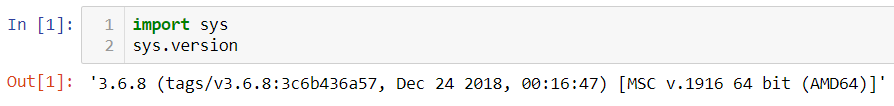
\includegraphics[width=0.9\textwidth]{imgs/Python_ver.PNG}
    \caption{Checking the installed version of Python.}
    \label{fig:pythver}
\end{figure}

\noindent To install Python, visit \url{https://www.python.org/} and download the installer for your Operating System.

\subsection{Python Package Dependencies}
The following packages are required dependencies for the \pkgname{} package. If you installed \pkgname{} through PIP, these dependencies should be installed automatically.

    \begin{itemize}
        \item \textbf{Pandas} $\geq$ v0.23
        \begin{itemize}
            \item \url{https://pandas.pydata.org}
        \end{itemize}
        \item \textbf{NumPy} $\geq$ v1.16
        \begin{itemize}
            \item \url{https://www.numpy.org}
        \end{itemize}
        \item \textbf{SciPy} $\geq$ v1.2
        \begin{itemize}
            \item \url{https://www.scipy.org}
        \end{itemize}
    \end{itemize}

\section{Optional Dependencies}
The following packages are optional dependencies for the \pkgname{} package. These dependencies will not be installed automatically when installing \pkgname{} with PIP, so they must be installed manually if needed.

\begin{itemize}
    \item \textbf{Fuzzy} $\geq$ v1.2.2
    \begin{itemize}
        \item This package is required for the Soundex corruption method. For more information about the package, visit \url{https://pypi.org/project/Fuzzy/}.
    \end{itemize}
    \item \textbf{Jupyter} $\geq$ v1.0.0
    \begin{itemize}
        \item This package is required to view and run the tutorial Jupyter notebook. For more information about Jupyter, visit \url{https://jupyter.org/}
    \end{itemize}
\end{itemize}

\section{Installation}

\subsection{PIP Method (Recommended)}
To install the package via PIP run the command:
\begin{verbatim}
    pip install git+git://github.com/cu-recordlinkage/ipprl_tools
\end{verbatim}
through a command-line interface.
\\
\\
\noindent This command will install the \pkgname{} package into your default Python environment. This command will also install the required dependencies (Pandas, NumPy, SciPy, etc) if they are not already installed. 

\subsection{GitHub Method}: 
The source code can also be cloned directly from GitHub using the following command from a command-line interface.

\begin{verbatim}
    git clone https://github.com/cu-recordlinkage/ipprl_tools
\end{verbatim}

\section{Usage}
\subsection{Importing the Package}
To use \pkgname{}, first import the \verb|synthetic| submodule. 
\begin{figure}[H]
    \centering
    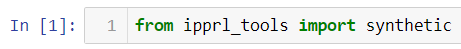
\includegraphics{imgs/Import}
    \caption{Importing \pkgname{}}
    \label{fig:my_label}
\end{figure}

\noindent This command will import all of the functions defined in the \verb|synthetic| submodule. If you only need a subset of the functions, you can specify the exact functions to import as well:

\begin{figure}[H]
    \centering
    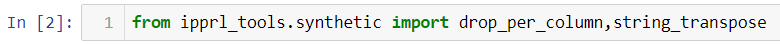
\includegraphics{imgs/Import2}
    \caption{Importing specific functions}
    \label{fig:my_label}
\end{figure}

\subsection{Data Prerequisites}
The synthetic data functions are designed to operate on Pandas DataFrame objects. Pandas DataFrame objects are data structures, similar to R dataframes, which contain data organized in named columns. 
\\
\\
\noindent Before using the synthetic data methods, first read the raw data in as a Pandas DataFrame. The example below shows reading a CSV file in using Pandas.
\\
\noindent For additional ways to import data using Pandas, refer to the Pandas Documentation here:
\\
\href{https://pandas.pydata.org/pandas-docs/stable/user_guide/io.html}{Pandas Documentation: IO}
\\

\begin{figure}[H]
    \centering
    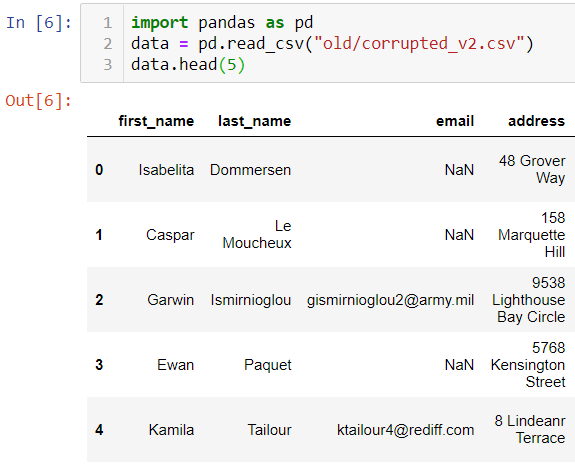
\includegraphics{imgs/PandasRead.png}
    \caption{Reading in a CSV file with Panda}
    \label{fig:my_label}
\end{figure}

\section{Corrupting Existing Data}
In order to make generating synthetic datasets easier, \pkgname{} provides a file a pre-made synthetic data, generated using Mockaroo (Link: \url{https://mockaroo.com/}).
\\
\noindent Using \pkgname{}, the user can automatically download this data, import it into their Python interpreter, and perform corruption using the corruption methods provided in \pkgname{}. 
\subsection{Downloading the Data}
To download the data, first import the \verb|get_data()| function from the \verb|utils.data| submodule of \pkgname{}.

\begin{figure}[H]
    \centering
    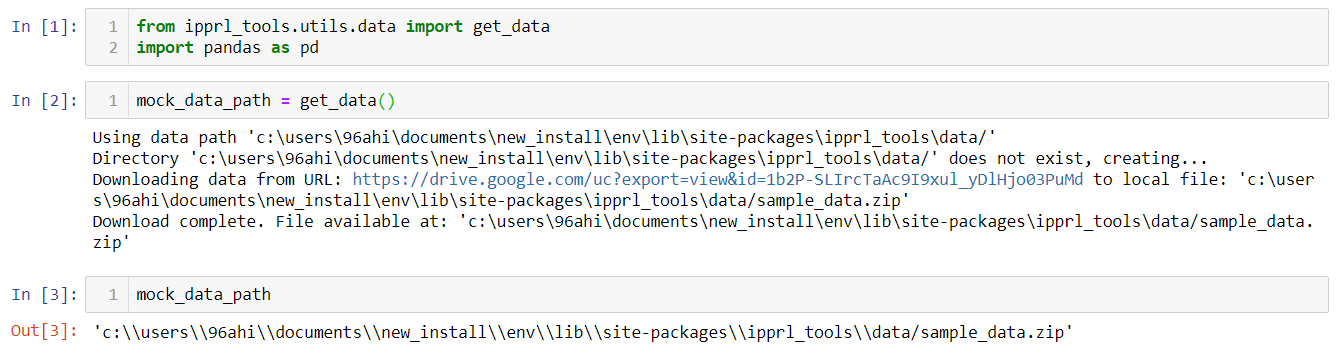
\includegraphics[width=0.9\textwidth]{imgs/mock_data1.PNG}
    \caption{Importing the \pkgname{} submodule, along with Pandas (So we can read the file in as a DataFrame).}
    \label{fig:my_label}
\end{figure}

\noindent In the above figure, \verb|get_data()| determines that the pre-made data bundle has not been downloaded before, so it creates a new directory and downloads the data. \verb|get_data()| returns the file path where the data bundle was downloaded. In future calls to \verb|get_data()|, the data path will be returned immediately without re-downloading the data unless the file is moved or deleted. 
\\
\\
\noindent After downloading the data bundle, we can read it in to a DataFrame using the \verb|read_pickle()| method from Pandas.

\begin{figure}[H]
    \centering
    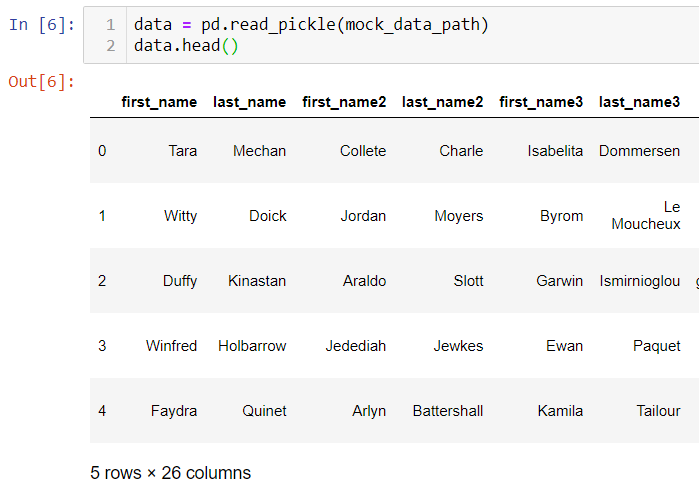
\includegraphics[width=0.8\textwidth]{imgs/mock_data2.PNG}
    \caption{Reading the data into a DataFrame using Pandas.}
    \label{fig:dataread}
\end{figure}

\noindent At this point, we are able to apply any corruption method desired to the DataFrame. 

\begin{figure}[H]
    \centering
    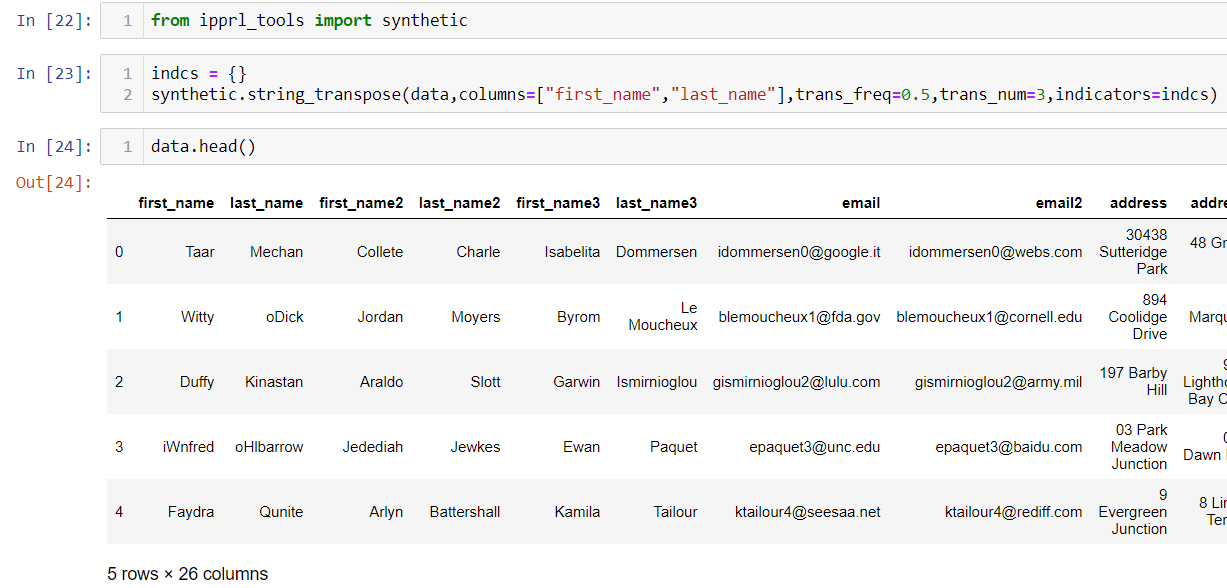
\includegraphics[width=0.9\textwidth]{imgs/mock_data3.PNG}
    \caption{Applying a String Transpose corruption to the mock data.}
    \label{fig:datacorrupt}
\end{figure}

\noindent In the following three cells we import the \verb|synthetic| sub-module of \pkgname{}, which contains all of the methods for data corruption.
We then apply a String Transpose corruption to the \verb|first_name| and \verb|last_name| columns of the data. 
\\
\\
\noindent After viewing, we can see that some of the values in \verb|first_name| and \verb|last_name| have been randomly transposed. 
\\
\\
\noindent For a complete overview of the synthetic data corruption methods and their usage, refer to the \textbf{\pkgname{} Documentation: Synthetic Data Corruption Tools} document, which contains information about the \verb|synthetic| sub-module of \pkgname.

\subsection{Splitting Data for Linkage}
One common use case for mock patient record data is testing the performance of linkage methods. To assist with this use case, \pkgname{} also provides a utility for splitting the data bundle (or your own dataset) into two equal-sized groups, with a user-specified amount of overlapping records.

\begin{figure}[H]
    \centering
    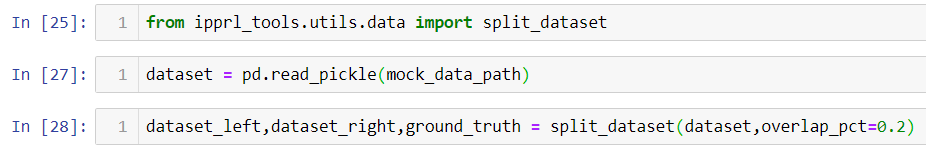
\includegraphics[width=0.9\textwidth]{imgs/mock_data4.PNG}
    \caption{Importing the \textit{split\_dataset()} function, and applying it on a DataFrame.}
    \label{fig:datasplit}
\end{figure}

\noindent In the above example, we read mock data path into a new DataFrame called \verb|dataset|, then call \verb|split_dataset(dataset,overlap_pct=0.2)| on the DataFrame. This call will split the data bundle into two equal-sized datasets, with 20\% of the records from \verb|dataset| appearing in both new datasets.
\\
\\
\noindent This function call returns two DataFrames (referred to in the example code as \verb|dataset_left| and \verb|dataset_right|). In addition, this function call returns \verb|ground_truth|, which is a list of tuples mapping IDs in \verb|dataset_left| to IDs in \verb|dataset_right|. These IDs are generated by the function, and are contained in the \verb|id| column of both \verb|dataset_left| and \verb|dataset_right|.

\begin{figure}[H]
    \centering
    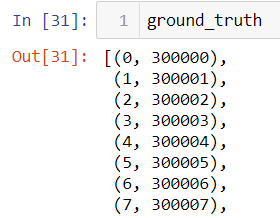
\includegraphics{imgs/mock_data5.PNG}
    \caption{View of \textit{ground\_truth}, which is a list of tuples of integers, mapping IDs from \textit{dataset\_left} to \textit{dataset\_right}.}
    \label{fig:groundt}
\end{figure}

\begin{figure}[H]
    \centering
    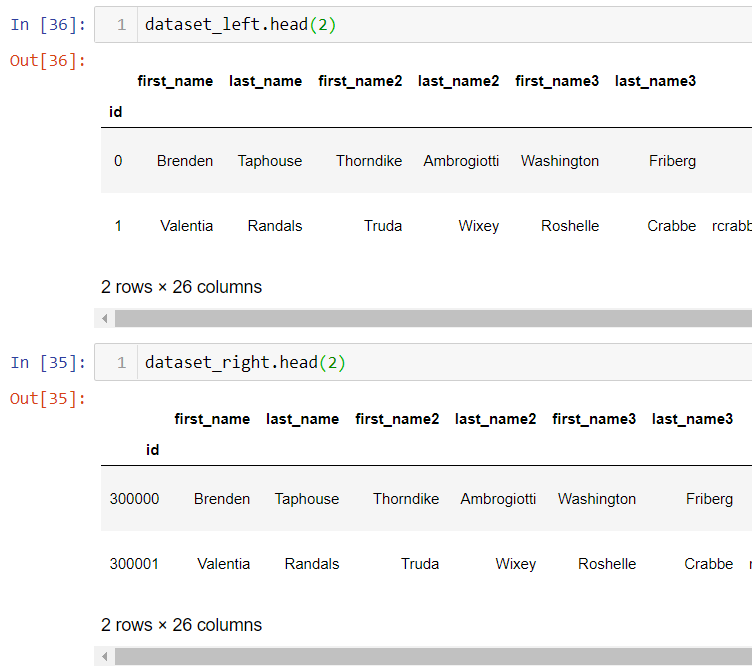
\includegraphics[width=0.9\textwidth]{imgs/mock_data6.PNG}
    \caption{Views of \textit{dataset\_left} and \textit{dataset\_right}. The \textit{id} is visible as the left-most column in both DataFrames.}
    \label{fig:datacomp}
\end{figure}

\noindent As is visible in Figures \ref{fig:groundt} and \ref{fig:datacomp}, the \verb|ground_truth| variable links the \verb|ID|s of matching records between \verb|dataset_left| and \verb|dataset_right|. 
\\
\\
\noindent After this process is complete, \verb|dataset_left| and \verb|dataset_right| can be corrupted and shuffled independently, then used as inputs for record linkage. When the linkage process is complete, the user can compare the results against the \verb|ground_truth| list to determine the performance of the linkage on the synthetic data.
\end{document}
